

\paragraph{} In this chapter we shall introduce and detail a prototype implementation of a modular, SGX-protected \textit{reference monitor} --- \textsc{Citadel}. First, its necessity will be motivated, and the challenges faced discussed. Then, the three-part architecture will be explained, relating various design decisions to the DIFC model it provides. A discussion about the architecture's performance and effectiveness is provided in §~\ref{sec:eval}.

\section{Motivation}
\paragraph{} Since its introduction in a 1972 report from Anderson~\cite{reference-monitor}, the reference monitor concept has time and again proved to be a reliable workhorse for a plethora of security models. It does not refer to any exact policy, nor limit itself to any particular implementation --- it's abstractness is one of its greatest strengths, reserving any judgement about what policy is \textit{appropriate} in a particular setting.~\cite{irvine-rm}

\paragraph{Fundamental Properties of a Reference Monitor}

\begin{itemize}
    \item \textit{Always invoked.} Every access to the system must be mediated to guarantee that adversaries are unable to bypass the system's security policies.
    \item \textit{Evaluable.} It ``must be small enough to be subject to analysis and tests, the completeness of which can be assured'';~\cite{reference-monitor} to be trustworthy, it must be \textit{auditable}, with, ideally, a restricted TCB.
    \item \textit{Tamper proof.} To ensure that an attacker cannot disable the access control and authorisation steps mandated by the security policy, the integrity of a reference monitor cannot be in question.
\end{itemize}

\paragraph{} No computer system is every completely secure, and Linux is no exception. Having grown by a 1.7 million lines of code (LoC) in the past year alone, now standing at 27.8 million LoC in total,\footnote{\url{https://www.theregister.com/2020/01/06/linux\_2020\_kernel\_systemd\_code/}} bugs are inevitable --- almost 2000 have been reported in the past year,\footnote{\url{https://bugzilla.kernel.org/}} and 662 \textit{severe} bugs are still outstanding.\footnote{\url{https://www.cvedetails.com/product/47/Linux-Linux-Kernel.html}} In this context we must question whether Linux alone can provide a reference monitor implementation the guarantees it requires,~\cite{Lipp2018MeltdownRK, 10.5555/2831143.2831164} thus motivating the use of SGX.

\paragraph{} Applying SGX to this problem brings two attractive benefits;
\begin{itemize}
    \item The system's IFC policy can be evaluable both during offline analysis and online using \textit{attestation}, helping other enclaves' confidence in the underlying system.
    \item SGX's hardware protections are very capable at defending a reference monitor's state, even if adversaries have ring-0 privilege or in the presence of a kernel bug.
\end{itemize}

\section{Challenges}

\begin{figure}[]
    \centering
    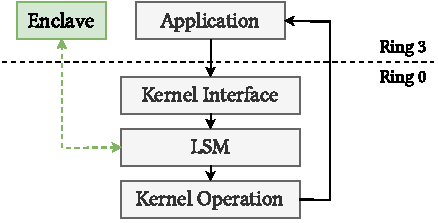
\includegraphics[width=0.48\linewidth]{figures/SGX-EnclaveIntegration.pdf}
    \caption{Abstract \textit{syscall} control flow route. Grey components show the natural Linux design. Green additions highlight the externalised enclave LSM component.}
    \vspace{5mm}
    \label{fig:sgx-abstract-integration}
\end{figure}

\paragraph{} The natural location for a reference monitor is embedded directly in the kernel, in the path of \textit{syscalls'} control flows --- this is provided by the LSM framework. \textit{CamFlow} does exactly this, silently tagging processes and other entities as they are encountered by the kernel, additionally providing an external LSM-interface for any active changes. However, as explained in §~\ref{sec:sgx-no-kernel-mode}, an SGX enclave is incompatible with this workflow as it cannot execute alongside kernel code. Thus a major, unavoidable consequence of this is that the reference monitor must be distributed across rings 0 and 3 --- an enclave \textit{policy} component, and an LSM for \textit{enforcement}.

\paragraph{} The disruption this change causes could have the potential to severely impact performance; Figure~\ref{fig:sgx-abstract-integration} highlights the significant change to overall control flow. Mostly notably, externalising part of the LSM to an enclave forces an additional pair of context switches for each \textit{syscall}.

\paragraph{} Given a ring-3 component is unavoidable, the question becomes how to minimise the overhead caused by its integration, all while maintaining \textit{safety} (every operation must be mediated). This problem is reminiscent of the ones that inspired the development of \textit{exokernels}~\cite{10.1145/224056.224076} --- both the drawbacks and opportunities of those approaches apply here.~\cite{10.1145/269005.266644} \textcolor{red}{More detail about why.}

\paragraph{} Two architectures, as illustrated in Figure~\ref{fig:sgx-integration}, were initially considered. 

\begin{enumerate}
    \item An \textit{isolated} extension of the LSM. Only the security implementation communicates with the \textit{policy} enclave, acting as a na\"{i}ve reimplementation of a fully self-contained LSM using an additional kernel module as a I/O relay.
    \item An \textit{integrated} userspace service, through which permission is \textit{requested} ahead of time and decisions stored in the LSM before being claimed. Back flow of information is facilitated asynchronously, but an additional kernel relay is not required.
\end{enumerate}



\begin{figure}[]
    \centering
    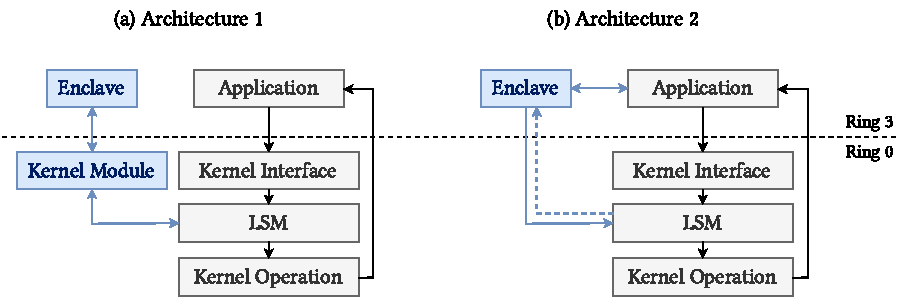
\includegraphics[width=0.98\linewidth]{figures/SGX-EnclaveIntegration-Design}
    \caption{}
    \vspace{2mm}
    \label{fig:sgx-integration}
    \vspace{5mm}
\end{figure}

\paragraph{}\textit{Architecture 1} can be implemented without changing the base IFC model presented in §~\ref{sec:ifc-modelling}, easing potential concerns regarding correctness and safety. However it adds significant overhead to the critical sections~\cite{Dubois1988SynchronizationCA} of core LSM functions, in most cases while the kernel holds locks for various objects being accessed.

\paragraph{} \textit{Architecture 2} is more flexible, requiring all negotiation be conducted ahead of time, importantly without leaving userspace: any overhead only impacts the application, leaving the kernel's critical sections to execute with minimal interference. A notable downside, however, is that the system's security model will need to be extended to accommodate the fact that \textit{policy decisions and enforcement are no longer one and the same}.


\clearpage
\begin{figure}[]
    \centering
    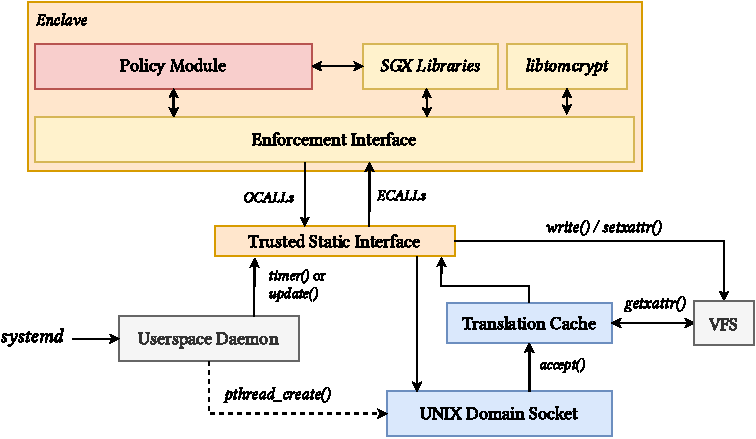
\includegraphics[width=\linewidth]{figures/EnclaveLayout.pdf}
    \caption{Abstract overview of an SGX enclave's protections.}
    \label{fig:sgx-basic}
\end{figure}